%%%%%%%%%%%%%%%%%%%%%%%%%%%%%%%%%%%%%%
%%%%%%%%%%%%%%%%%%%%%%%%%%%%%%%%%%%%%%
% Do not edit the TeX file your work
% will be overwritten.  Edit the RnW
% file instead.
%%%%%%%%%%%%%%%%%%%%%%%%%%%%%%%%%%%%%%
%%%%%%%%%%%%%%%%%%%%%%%%%%%%%%%%%%%%%%





\newcommand{\EoneNumObs}{1,000}


We generated $\EoneNumObs$ observations.  They looked like a mess,
as you can see in \figref{eone_scatter}.


\begin{knitrout}
\definecolor{shadecolor}{rgb}{0.969, 0.969, 0.969}\color{fgcolor}\begin{figure}[!h]

{\centering 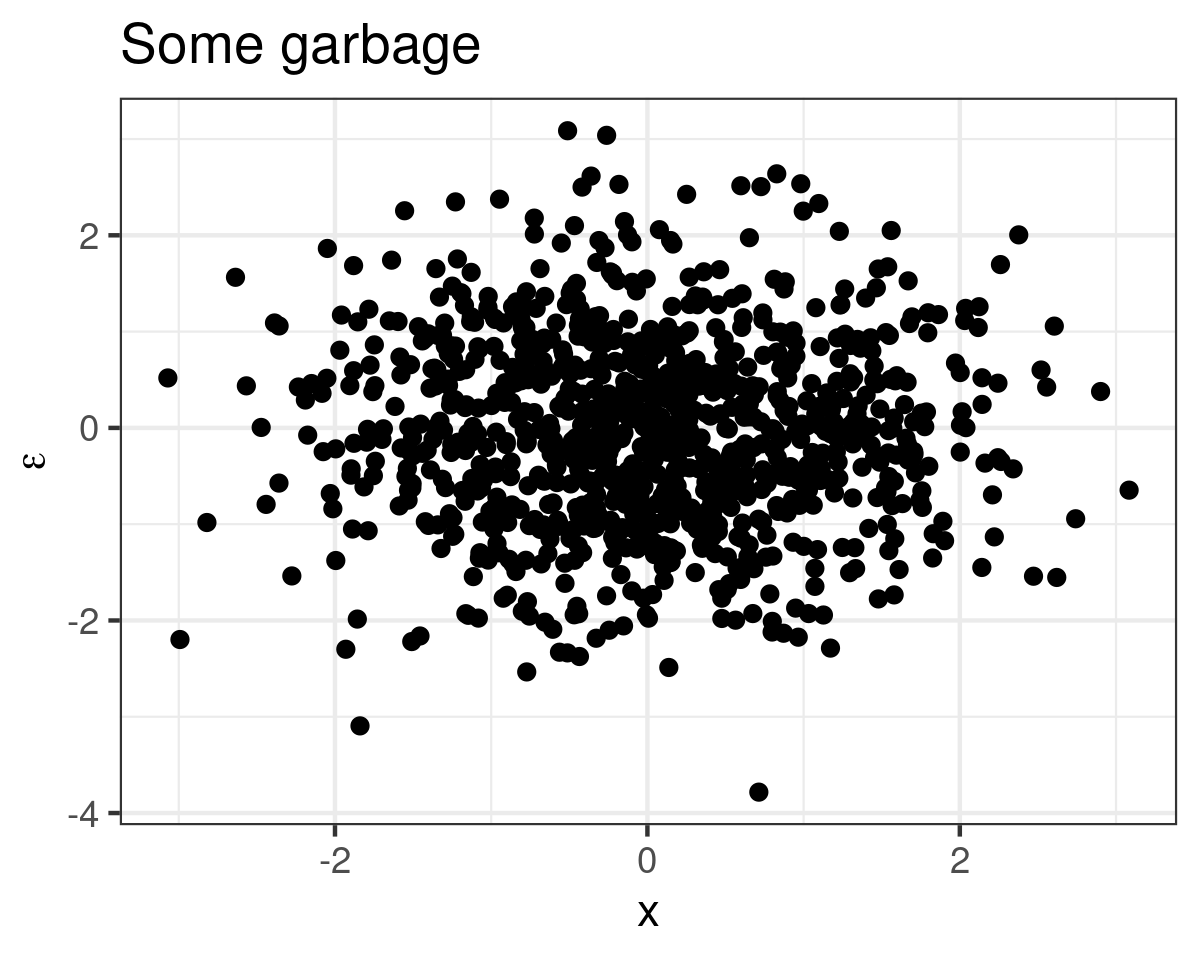
\includegraphics[width=0.980\linewidth,height=0.784\linewidth]{figure/eone_scatter-1} 

}

\caption[It's nice to have a long figure caption that allows easy access to latex stuff like there were $\EoneNumObs$ draws of $x$ and $\epsilon$ that went into this plot]{It's nice to have a long figure caption that allows easy access to latex stuff like there were $\EoneNumObs$ draws of $x$ and $\epsilon$ that went into this plot.}\label{fig:eone_scatter}
\end{figure}


\end{knitrout}

And \figref{eone_hist} as well.  What garbage.


\begin{knitrout}
\definecolor{shadecolor}{rgb}{0.969, 0.969, 0.969}\color{fgcolor}\begin{figure}[!h]

{\centering 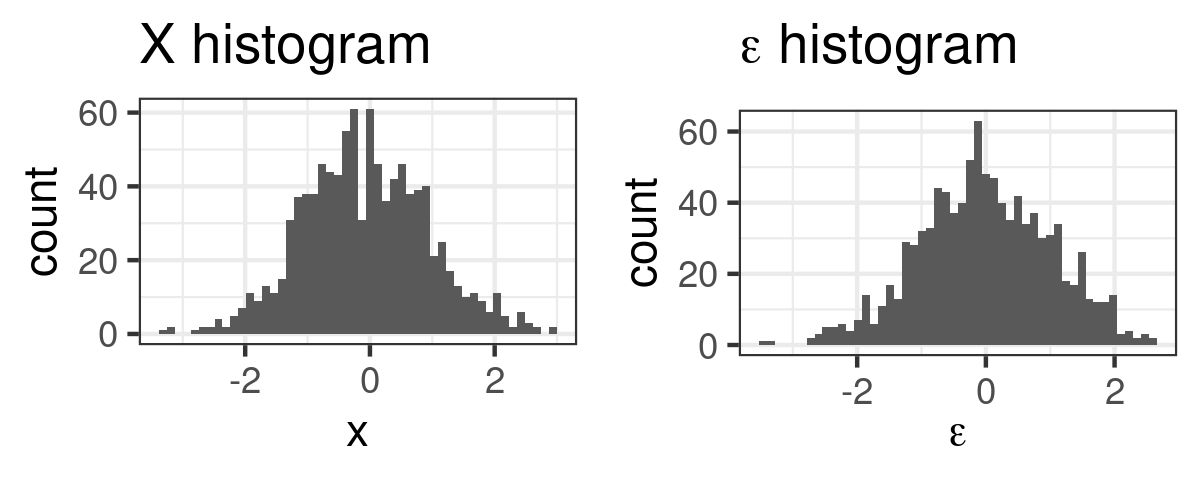
\includegraphics[width=0.980\linewidth,height=0.392\linewidth]{figure/eone_hist-1} 

}

\caption[You can reuse this variable for other captions]{You can reuse this variable for other captions.}\label{fig:eone_hist}
\end{figure}


\end{knitrout}
%
